Here a survey of the theory behind the work will be exposed but in a briefly matter. The Markov Decision Process section was based on  the book \cite{RFIntroduction} and on \cite{UCBerkley}. The Neural Network section was derived from \cite{NNs}.

\section{Markov Decision Processes}


\renewcommand{\vec}[1]{\mathbf{#1}}

A MDP (Markov Decision Process) is a mathematical model of the reinforcement learning problem. It is composed by an agent, the decision maker, and the thing it interacts with, the environment. These two interact continually, with the environment presenting a situation to the agent in the form of a state, and the agent selecting an action in regards to this state. This same environment also presents the agent with numerical rewards for each state accessed, the goal of the agent is to maximize the sum of these rewards by making good choices of actions.

In short, the MDP is defined by:
\begin{itemize}
	\item A set of states $ s \in S $
	\item A set of actions $ a \in A $
	\item A transition function $ T\left(s, a, s^\prime\right) $
	\begin{itemize}
		\item Probability that $a$ from $s$ leads to $s^\prime$, i.e., $P\left(s^\prime\mid s, a\right) $
		\item Also called the model of the dynamics
	\end{itemize}
	\item A reward function $R\left(s\right)$
	\item A start state
	\item Maybe a terminal state
\end{itemize}

For each time step, the environment returns its current representation in the form  of a state $s$. The agent then selects an action and the transition function $ T\left(s, a, s^\prime\right) $ returns the probability of reaching state $s^\prime$ from state $s$ given the action chosen. On the next time step, the agents finds itself on a new state.

\subsection{Important Concepts}
Here a list of important concepts of a MDP is shown.
\subsubsection{Reward Function}
At each reached state, the agent accumulates a reward returned by a reward function $R\left(s\right)$. The purpose of this functions is to guide the agent, good states are scored with positive  values, while bad states are scored with negative values. By making the agent act on the desire of maximizing his reward score, the agent will act optimally as  it is intentioned.


\subsubsection{Transition Function}
The MDP is not necessarily deterministic, after an agent chooses an action the next state is ruled by a probability distribution. The transaction function $ T\left(s, a, s^\prime\right)$ return the probability that an agent in state $s$ performing action $a$ will land in state $s^\prime$.




\subsubsection{Discounting}
In a MDP, it's reasonable to maximize the sum of rewards but it's also reasonable to make preference over rewards now than later. One solution is to make rewards decay exponentially in value. So for each episode, all rewards available are multiplied by a $\gamma$ factor as illustrated by \ref{Discounting}. This factor is called discount factor.

\begin{figure}[h]
	\centering
	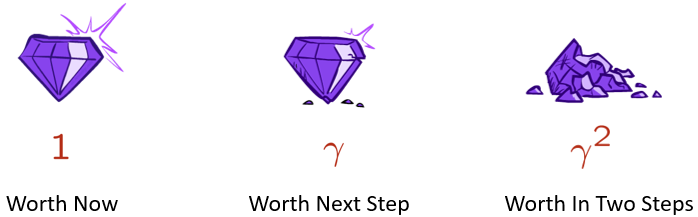
\includegraphics[width=1.0\textwidth]{Cap3/Discount}
	\caption{Illustrating of the discount factor, image from http://ai.berkeley.edu}
	\label{Discounting}
\end{figure}



\subsubsection{Utility}
Utility is, by definition,  the sum of the discounted rewards for a given trajectory of the agent.
\begin{equation} \label{Utility}
G_t \doteq R_{t+1} + \gamma\,R_{t+2} + \gamma^{2}\,R_{t+3} + \dotsm = \sum_{k = 0}^{\infty}\gamma^{k}\,R_{t+k+1}
\end{equation}
In recursive form:
\begin{equation} \label{UtilityRec}
G_t \doteq R_{t+1} + \gamma\,G_{t+1}
\end{equation}

\begin{figure}[h]
	\centering
	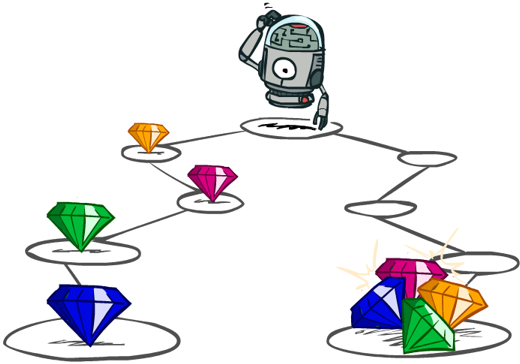
\includegraphics[width=0.6\textwidth]{Cap3/Reward}
	\caption{Illustration of a Reward and Utility, image from http://ai.berkeley.edu}
	\label{Reward}
\end{figure}

\subsubsection{Policy}

For MDPs, an \textit{optimal policy} $\pi^*: S \to A $ is desired. To put it simply, a \textit{policy} $\pi$ works as a map of instructions. Given a state $s$, the policy return which action $a$ to take. Therefore, an optimal policy has an action for each state that maximizes the expected utility when followed.

\begin{figure}[h]
	\centering
	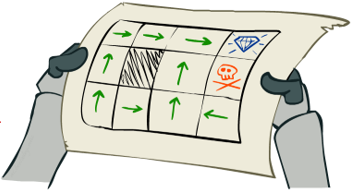
\includegraphics[width=0.6\textwidth]{Cap3/Policies}
	\caption{Illustration of a policy, image from http://ai.berkeley.edu}
	\label{Policies}
\end{figure}

\subsubsection{Value Function}
The \textit{value function} of a state $s$ under a policy $\pi$, denoted $v_{\pi}\left(s\right)$, is the expected return when starting in s and following $\pi$ thereafter. Formally:
\begin{equation} \label{ValueFunction}
v_{\pi}\left(s\right) \doteq \mathbf{E}_{\pi}\left[G_{t}\mid\,S_{t} = s\right]
\end{equation}
where $\mathbf{E}_{\pi}$ represents the expected value of a random variable given that the agent follows policy $\pi$.

\subsubsection{Q-State}
A Q-State is a tuple formed by a state $s$ and an action $a$.

\subsubsection{Action Value Function}
Just like the Value Function, the \textit{action value function} defines value for the Q-States. The value of taking action $a$ in state $s$ under the policy$\pi$, denoted $q_{\pi}\left(s,a\right)$, as the expected return starting from $s$, taking the action $a$, and thereafter following policy $\pi$. Formally:
\begin{equation} \label{ActionValueFunction}
q_{\pi}\left(s,a\right) \doteq \mathbf{E}_{\pi}\left[G_{t}\mid\,S_{t} = s,A_{t} = a\right]
\end{equation}




\subsection{The Bellman Equations}

\subsubsection{Optimal Quantities}

\begin{itemize}
	\item $V^*\left(s\right)$  is the expected utility starting in $s$ and acting optimally.
	\item $Q^*\left(s,a\right)$ is the expected utility starting out having taken action $a$ from state $s$ and (thereafter) acting optimally.
	\item $\pi^*\left(s\right)$ returns the optimal action from state $s$
\end{itemize}

\subsubsection{The Equations}

\begin{equation} \label{Bellman1}
V^*\left(s\right) = \underset{a}{\text{max}}\,Q^*\left(s,a\right)
\end{equation}

\begin{equation} \label{Bellman2}
Q^*\left(s,a\right) = 
\end{equation}

\subsection{About Solving It}
To make things clear, the solution required is the optimal policy, the set of instructions that maximizes the utility. If the transition function is know and well defined than the solution is easily found by means of dynamic programming, no reinforcement learning involved. Of course, in the real world, this transition function cannot be know a priori, that's where reinforcement learning comes.

The most basic reinforcement learning algorithms have the agent updates states values in a series of trainings, multiple sessions of sampling substitutes the transition function. The idea is to have the agent explore the environment by doing, at first, random actions; but as time passes and almost all states are decently evaluated, it progressively abandons the random nature of exploration in favor of a greedy behavior in which the agent chooses the action that will return the best benefit, ergo the best reward.

In Q-Learning algorithm, for example, the Q-States values are updated by the following expression \ref{Qupdate}:
\begin{equation} \label{Qupdate}
Q\left(s,a\right) \leftarrow \left(1 - \alpha\right)Q\left(s,a\right) + \left(\alpha\right)\left[r + \gamma\,\underset{a^\prime}{\text{max}Q\left(s^\prime,a^\prime\right)} \right]
\end{equation}
where $\alpha$ is a factor that averages the current value with the next value. The expression is very intuitive, the Q value is updated by an average between its current value and the reward the state gives plus the discounted maximum Q-Value accessible by the current state.

By doing a series of training, the Q-Values will converge and then the optimal policy may be extracted by using \ref{OptimalPolicy}:
\begin{equation} \label{OptimalPolicy}
\pi^*\left(s\right) = \underset{a}{\text{arg max}}\;Q^*\left(s,a\right)
\end{equation}

\subsection{The Problem With The Tabular Solution}
Q-Learning solves the MDP but it's solution is brute force styled (Without optimizations that is). That's because  the algorithm contemplates all states and it's possible actions without any scrutiny. For real world problems, that's not computational feasible. For instance, Go has a number of possible situations greater than the number of atoms in the whole observable universe.

A great improvement is to make state approximations.  For example, if you look at a Pac-Man game, each configuration on the board is a different state, move a ghost or Pac-Man just a bit and a whole new state is reached. The insight here is that some states are actually very close to each other. All states that has Pac-Man moving close to a ghost (which results in PacMan's death) are equally bad states to be avoided \ref{fig:Pacman}. So there is actually no need to register all these similar states if you can extract crucial information from them and hereby decide if they are bad or not. What is wanted is that the machine, by looking at these relevant informations, learns what they mean in order to classify states.

\begin{figure}[h]
	\begin{subfigure}{.5\textwidth}
		\centering
		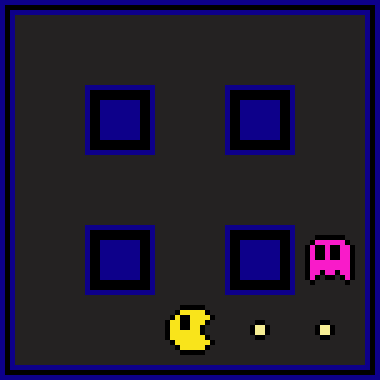
\includegraphics[width=.8\linewidth]{Cap3/pacman1}
		\caption{1a}
		\label{fig:sfig1}
	\end{subfigure}%
	\begin{subfigure}{.5\textwidth}
		\centering
		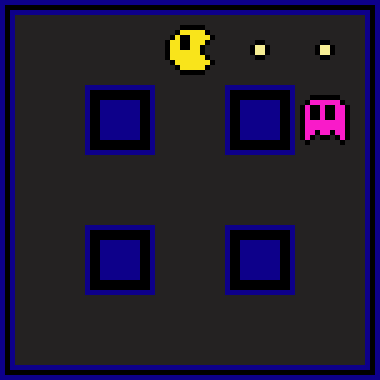
\includegraphics[width=.8\linewidth]{Cap3/pacman2}
		\caption{1b}
		\label{fig:sfig2}
	\end{subfigure}
	\caption{The two Pac-Man states  are different yet for what it matters they are both states to be avoided in equal magnitude.}
	\label{fig:Pacman}
\end{figure}

The role of function approximation belongs to Neural Networks in Deep Learning.

\section{Neural Networks}

A Neural Network is a learning model whose goal is essentially function approximation. For example, for a classifier, $y = f^*\left(x\right)$ maps an input $x$ to a category $y$. A neural network defines a mapping $y = f\left(x,\theta\right)$ and learns the value of the parameters $\theta$ that result in best function approximation.
They are called networks because they are commonly represented by composing together many different functions. The model is illustrated by a directed acyclic graph describing how the functions are composed together. For example, there could be three functions $f_{1}$, $f_{2}$ and $f_{3}$ connected in a chain, to form $f\left(x\right) = f_{3}\left(f_{2}\left(f_{1}\left(x\right)\right)\right)$.

\subsection{Neurons}

Neurons are the single unit from a Neural Network. They are an abstraction of a vector of \textit{weights} $\vec{w}$ and a number $b$ called \textit{bias}. Upon receiving an input $\vec{x}$, the neuron outputs:
\begin{equation}\label{Neuron}
z = \vec{w}\boldsymbol{\cdot}\vec{x} + b
\end{equation}

Actually, because the values of $\vec{w}$ and $b$ are supposed to be changed by a learning process, it is important that the output changes in linear form in relation to them so these changes may actuate smoothly. To achieve it, the \textit{sigmoid function} is often used, the final output is therefore:
\begin{equation}\label{}
\text{Neuron output} = \sigma\left(z\right) = \dfrac{1}{1 + e^{-z}}
\end{equation}
where $z$ is extracted from \ref{Neuron}.

\subsection{The Network}
In graph representation, a neuron is a vertex and each incoming edge is a weight in the weight vector $\vec{w}$. Networks are composed of layers of neurons, the first layer receives the initial input while the subsequent layers receive input from their predecessor layer. The last layer returns the final output.

\subsection{Cost Function and Gradient Descent}
After a final output is received from the last layer, there is need to check how adequate it is and at the some time use this result to better balance the weights and biases. For that, it is defined a \textit{cost function}. The simplest example is the \textit{quadratic cost function}:
\begin{equation}\label{CostFunction}
C\left(w,b\right) \equiv \frac{1}{2n}\,\sum_{\vec{x}}\norm{y\left(\vec{x}\right) - \vec{a}}^{2}
\end{equation} 
Here,$y\left(x\right)$ denotes the desired output, $w$  the collection of all weights in the network, $b$ all the biases, $n$ is the total number of training inputs, $\vec{a}$ is the vector of outputs from the network when $\vec{x}$ is input, and the sum is over all training inputs, $\vec{x}$.

The more the desired output is different from the received output, the higher the cost function value will be.Therefore, the true objective is to manipulate the values of weights and biases in order to shrink the cost function returning value. This is achieved by \textit{gradient descent} \cite{}. By calling $\vec{W}$ the collection of weights and biases, the update rule would be:
\begin{equation}\label{GradientDescent}
\vec{W}^\prime = \vec{W}  - \epsilon\;\frac{\nabla\,C\left(\vec{W}\right)}{\norm{\nabla\,C\left(\vec{W}\right)}}
\end{equation}
where $\epsilon$ is a step size.

The algorithm that applies this update rules efficiently are called \textit{Back Propagation Algorithms}

\subsection{Back Propagation}
Back Propagation allows the calculation of $\dfrac{\partial C_x}{\partial w}$ and $\dfrac{\partial C_x}{\partial b}$ of a single training sample. Then $\dfrac{\partial C_x}{\partial w}$ and $\dfrac{\partial C_x}{\partial b}$ is recovered by averaging over the samples.

\subsubsection{Notation}
\begin{itemize}
	\item $w_{jk}^{l}$ denotes the weight for the connection from the $k^{th}$ neuron in the $\left(l-1\right)^{th}$ layer to the $j^{th}$ neuron in the $l^{th}$ layer.
	\item $b_{j}^{l}$ is the bias of the $j^{th}$ neuron in the $l^{th}$ layer.
	\item $z_{j}^{l}$ is the output of the $j^{th}$ neuron in the $l^{th}$ layer \textbf{before} being processed by the sigmoid function. 
	\item $a_{j}^{l}$ is the output of the $j^{th}$ neuron in the $l^{th}$ layer \textbf{after} being processed by the sigmoid function, ergo $\sigma\left(z\right)$
\end{itemize}

\subsubsection{Neuron Error Definition}
A change $\Delta z_{j}^{l}$ in $z_{j}^{l}$ propagates through the layers, causing the overall cost to change by an amount  $\frac{\partial C_x}{\partial z_{j}^{l}}\Delta z_{j}^{l}$. The higher the value of $\frac{\partial C_x}{\partial z_{j}^{l}}$, the more the cost function can be adjusted, if it is low than the neuron cannot  improve the cost function by much. Therefore, in an heuristic sense,  $\frac{\partial C_x}{\partial z_{j}^{l}}$ works as a measure of error in the neuron. The \textit{neuron error} is than defined as:
\begin{equation}\label{NeuronError}
\delta_{k}^{l} \equiv \frac{\partial C_x}{\partial z_{j}^{l}}
\end{equation}
 $\vec{\delta^l}$ will denote the vector of errors associated with layer $l$. Back propagation allows the computing of $\vec{\delta^l}$ for every layer, and then relating those errors to the quantities of real interest, $\dfrac{\partial C_x}{\partial w}$ and $\dfrac{\partial C_x}{\partial b}$.
 \subsubsection{Back Propagation Equations}
 First there is need for an equation for the error of the nodes in the last layer, that will serve as a base for the propagation. \textbf{Under the definition from \ref{NeuronError} and by applying the chain rule from Calculus, the neuron error for the last layer nodes is:}
 \begin{equation}\label{LastLayerError}
 \delta_{k}^{L} = \frac{\partial C_x}{\partial a_{j}^{L}}\,\sigma^{\prime}\left(z_{j}^{L}\right)
 \end{equation}
 where $L$ represents the last layer number. It may be important to note that $\frac{\partial C_x}{\partial a_{j}^{L}}$ should be easy to compute which is the case for the quadratic cost function, other cost functions should maintain this property as well.
 A better representation of \ref{LastLayerError} is in matrix form:
 \begin{equation}\label{BP1}
 \vec{\delta^{L}}  = \nabla_{a}C_{x}\odot\sigma^{\prime}\left(\vec{z^L}\right)
 \end{equation}
 where $\odot$ represents the Hadamart Product (CITAR).
 
 \textbf{Next, an equation for the error $\vec{\delta^{l}}$ in terms of the error in the next layer, $\vec{\delta^{l+1}}$:}
 \begin{equation}\label{BP2}
 \vec{\delta^{l}} = \left(\left(w^{l+1}\right)^{T}\vec{\delta^{l+1}}\right)\odot\sigma^{\prime}\left(z_{j}^{L}\right),
 \end{equation}
 where $\left(w^{l+1}\right)^{T}$ is the transpose of the weight matrix $\left(w^{l+1}\right)$ for the $\left(l+1\right)^{th}$ layer. Using these two equations, \ref{BP1} and \ref{BP2}, the algorithm can compute all neuron errors. Now what is left is how to calculate $\frac{\partial C_x}{\partial w}$ and $\frac{\partial C_x}{\partial b}$ using these errors.
 
 \textbf{An equation for the rate of change of the cost with respect to any bias in the network:}
 \begin{equation}
 \label{BP3}
 \frac{\partial C}{\partial b^l_j} =
 \delta^l_j.
 \end{equation}


 \textbf{An equation for the rate of change of the cost with respect to any weight in the network:}
 \begin{equation}\label{BP4}
 \frac{\partial C}{\partial w^l_{jk}} = a^{l-1}_k \delta^l_j.
 \end{equation}
 
 So by using equations \ref{BP1}, \ref{BP2}, \ref{BP3} and \ref{BP4}; you can compute $\nabla\vec{W}$ which represents the vector that contains all  partial derivatives of weights and biases together. Finally, by using \ref{GradientDescent} you can update all weights and biases for a single training.
 
 \subsubsection{Neural Networks in Reinforcement Learning}
 This section is to point out briefly that in reinforcement learning there is no actually correct output $y\left(x\right)$ used in the cost function \ref{CostFunction}. The \textit{reward} concept substitutes the error one. So in reinforcement learning, the neural network tuning algorithms  take in another form which will be presented next.
 
 (citar michal neuron netowrks)
 
 \section{Policy Gradient Methods, PPO}
 
 Q-Learning is an \textit{action-value} method, the actions are chosen by evaluating the action value in a given state. A \textit{policy gradient} method learns a parameterized policy that cant select actions without consulting a value function.
 A value function may still be used to learn the policy parameter, but is not required for action selection.
 
 \subsection{Notation and Concepts}
 Here are some new basic concepts about policy learning.
 \subsubsection{The parameters $\bm{\theta}$}
 The policy parameter vector is $\bm{\theta} \in \mathbb{R}^{d^\prime}$ thus $\pi\left(a\mid s,\vec{\theta}\right) = \mathbb{P}\left\{A_t = a\mid S_t = s, \bm{\theta}_t = \bm{\theta}\right\}$ represents the probability that action $a$ is taken at time $t$ given that the environment is in state $s$ at time $t$ with parameter $\bm{\theta}$. This parameter $\bm{\theta}$  vector is the weights and biases of a neural network.
 
 \subsubsection{The Score Function}
 
 Learning the policy parameter is based on the gradient of some scalar performance measure $J\left(\bm{\theta}\right)$ with respect to the policy parameter. This function is called \textit{score function} as the aim is to maximize it (unlike the cost function). Therefore, their updates approximate gradient ascent in $J$:
 \begin{equation}
 \bm{\theta_{t+1}} = \bm{\theta_t} + \alpha\widehat{\nabla J\left(\bm{\theta_t}\right)}
 \end{equation}
 where $\widehat{\nabla J\left(\bm{\theta_t}\right)}$ is a stochastic estimate whose expectation approximates the gradient
 of the performance measure with respect to its argument $\bm{\theta_t}$.
 
 \subsection{Policy Approximation and its Advantages}
 
 Policy gradient offer advantages that justify its use, in general these methods are often better than value based ones. Here are the main advantages:
 
 \begin{itemize}
 	\item Q-Learning cannot learn stochastic policies, a necessity in some environments. This also means that it needs its own exploration strategy which makes the process more inefficient.
 	\item Q-Learning cannot handle continuous actions while policy gradient can.
 	\item Policy gradient work directly at the desired answer and not implicitly like Q-Learning, the result is that Policy Gradient turns out to be faster to execute.
 \end{itemize}

\subsection{Policy Gradient Vanilla}
Sparing the details that can be found on \cite{RFIntroduction}, here is the update algorithm for Policy Gradient Method in its most basic form:

\begin{algorithm}
	\caption{Policy Gradient Vanilla}\label{PGVanilla}
	\begin{algorithmic}[1]
		\Procedure{Reinforcement}{$\pi,\alpha$}
		\State Initialize policy parameter $\bm{\theta_{t+1}}$
		\While{$True$}
		\State Generate an episode $S_0,A_0,R_1,\dots,S_{T-1},A_{T-1},R_T$ following the policy $\pi$
		\While{$t$ is not $T$}
		\State $G \gets \sum_{k = t+1}^{T}\gamma^{k-t-1}R_k$
		\State $\bm{\theta} \gets \bm{\theta} + \alpha\gamma G_t\nabla_{\theta}\ln{\pi\left(A_t\mid S_t,\bm{\theta_t}\right)}$
		\State $t \gets t + 1$
		\EndWhile\label{time}
		\EndWhile\label{forever}
		\EndProcedure
	\end{algorithmic}
\end{algorithm}

where $\gamma$ is the discount factor and $\alpha$ is the step size.
 
\subsubsection{Issues with the Vanilla Version}

\begin{itemize}
	\item \textbf{Full episodes are needed:} The first step on the algorithm proposed requires that an episode be first generated, that is a problem as these generations might be costly.
	\item \textbf{High gradient variance:}  The episode generated is stochastic leading to high variance in the results, the vanilla version does nothing to account for that problem.
	\item \textbf{Exploration} Even with the policy represented as probability distribution, there is a high chance that the agent will converge to some locally-optimal policy and stop exploring the environment.
\end{itemize}

The high variance issue is addressed in the Actor Critic family of algorithms.

\subsection{Actor Critic}

The problem of high variance in the vanilla version comes from the fact that  the value $G$ is used in respect to the current episode with no regards to the other $G$ values calculated on other episodes. The Actor-Critic method adds the idea of an \textit{advantage function}:
\begin{equation}
\delta = G_{t:t+1} - \gamma \hat{v}\left(S_t,\bm{w}\right) \\
\end{equation}

where  $\hat{v}\left(S_t,\bm{w}\right)$ represents the current estimative of the utility of state $s$ approximated by the parameters vectors $\bm{w}$. Now there is no need to generate the whole episode to start the training, the updates are executed by each step of the episode. Furthermore, the variance is mitigated as the updates are applied under a current prediction of the state utility. Substituting the $G$ value by the recursive formula:
\begin{equation}
\delta = R_{t+1} + \gamma\hat{v}\left(S_{t+1},\bm{w}\right) - \hat{v}\left(S_t,\bm{w}\right)
\end{equation}

Now there is a presence of two neural networks, one for the policy and one for the reward values for each state. Of course both needs to be updated. Here follows the whole algorithm:

\begin{algorithm}
	\caption{One-Step Actor Critic}\label{ActorCritic}
	\begin{algorithmic}[1]
		\Procedure{Actor Critic}{$\pi,\alpha^{\bm{w}},\alpha^{\bm{\theta}}$}
		\State Initialize policy parameter $\bm{\theta_{t+1}}$ and state-value weights $\bm{w}$
		\While{$True$}
		\State Initialize $S$
		\State $I \gets 1$
		\While{$S$ is not terminal}
		\State Extract action $A$ from the policy $\pi\left(\cdot\mid S,\bm{\theta}\right)$
		\State Take action $A$, observe $S^\prime$, $R$
		\State $\delta = R + \gamma\hat{v}\left(S_{t+1},\bm{w}\right) - \hat{v}\left(S_t,\bm{w}\right)$
		\State $\bm{w} \gets \bm{w} + \alpha^{\bm{w}}\delta\nabla_{w}\hat{v}\left(S,\bm{w}\right)$
		\State $\bm{\theta} \gets \bm{\theta} + \alpha^{\bm{\theta}}I\delta\nabla_{\theta}\ln{\pi\left(A_t\mid S_t,\bm{\theta_t}\right)}$
		\State $I \gets \gamma I$
		\State $S \gets S^\prime$
		\EndWhile\label{time2}
		\EndWhile\label{forever2}
		\EndProcedure
	\end{algorithmic}
\end{algorithm}

\subsection{Proximal Policy Optimization (PPO)}

Having a fixed step-size is not optimal, if the size of the step is too small than the training is too slow but if the sizes are too large the algorithms becomes unstable, changing the policy too much in each step. PPO aims to optimize this concept.

\subsubsection{Replacing the log}
So far in the Actor Critic we had:
\begin{equation}
J_{\bm{\theta}} = \mathbb{E}_t\left[\ln{\pi\left(A_t\mid S_t,\bm{\theta_t}\right)}\delta_t\right]
\end{equation}
The PPO paper (REFERENCIAR PAPER) suggests:
\begin{equation}
J_{\bm{\theta}} = \mathbb{E}_t\left[\dfrac{\pi\left(A_t\mid S_t,\bm{\theta_t}\right)}{\pi_{old}\left(A_t\mid S_t,\bm{\theta_t}\right)}\delta_t\right]
\end{equation}
so we define:
\begin{equation}
r_t\left(\bm{\theta}\right) \equiv \dfrac{\pi\left(A_t\mid S_t,\bm{\theta_t}\right)}{\pi_{old}\left(A_t\mid S_t,\bm{\theta_t}\right)}
\end{equation}
to simplify the notation.

\subsubsection{The Clipped Surrogate Objective}
By using $r_t\left(\bm{\theta}\right)$ the samples become more powerful in updating the values but this new potential may be exaggerated, if the probability of the new policy is way higher than the probability of the old policy than the size step may be too large. What is needed is a way to bound this steps:

\begin{equation}
J\left(\bm{\theta}\right) = min\left(r_t\left(\bm{\theta}\right)\delta_t,clip\left(r_t\left(\bm{\theta}\right),1-\epsilon,1 +\epsilon\right)\delta_t\right)
\end{equation}

\subsubsection{The Final Score Function}

This algorithm is an optimization of the Actor Critic model, hence it still estimates $v\left(s\right)$ values and is constituted of 2 neural networks, one to compute the policy parameters and the other for the critic values. The score function of the algorithm is:

\begin{equation} \label{eq:finalppoloss}
J^{CLIP + VF + S}(\boldsymbol{\theta}) = \mathbb{E}_{t}[J^{CLIP}(\boldsymbol{\theta}) - c_{1} J^{VF}(\boldsymbol{\theta}) + c_{2}S[\pi_{\boldsymbol{\theta}}](s_{t})].
\end{equation}

$J^{CLIP + VF + S}$ denotes the clipped surrogate loss detailed earlier. The second term, $J^{VF}$ is the squared loss from prediction of value function and its value computed by the samples collected. Thus, this term aims to train the Critic network. The third term, denotes a entropy term to ensure sufficient exploration (CITAR ARTIGO Q NEM O LUCK FEZ)

\subsubsection{Multiple epochs for policy updating}

Unlike vanilla policy gradient methods, and because of the Clipped Surrogate Objective function, PPO allows you to run multiple epochs of gradient ascent on your samples without causing destructively large policy updates. This allows you to squeeze more out of your data and reduce sample inefficiency.

PPO runs the policy using N parallel actors each collecting data, and then it samples mini-batches of this data to train for K epochs using the Clipped Surrogate Objective function.

\begin{algorithm}
	\caption{PPO}\label{PPO}
	\begin{algorithmic}[1]
		\Procedure{PPO}{}
		\For{\texttt{iteration} = 1,2,$\dots$ do}
			\For{\texttt{iteration} = 1,2,$\dots$,N }
				\State Run policy $\pi_{\bm{\theta_{old}}}$ in environment for $T$ time steps
				\State Compute advantage estimates $\hat{A}_1,\dots,\hat{A}_T$
			\EndFor
		\State Optimize surrogate $J$ with respect to $\bm{\theta}$ with K epochs and minibatch size $M \leq NT$
		\State $\bm{\theta_{old}} \gets \bm{\theta}$
		\EndFor
		\EndProcedure
	\end{algorithmic}
\end{algorithm}

The new part is that they are able to run K epochs of gradient ascent on the trajectory samples. As they state in the paper, it would be nice to run the vanilla policy gradient optimization for multiple passes over the data so that you could learn more from each sample. However, this generally fails in practice for vanilla methods because they take too big of steps on the local samples and this wrecks the policy. PPO, on the other hand, has the built-in mechanism to prevent too much of an update


 
 
 











